%!TEX root = ../report.tex
\chapter{Introduction}

\textit{P2P is a class of applications that takes advantage of resources -- storage, cycles, content, human presence -- available at the edges of the Internet. Because accessing these decentralized resources means operating in an environment of unstable connectivity and unpredictable IP addresses, P2P nodes must operate outside the DNS system and have significant or total autonomy from central servers.} -- Clay Shirky~\cite{Shirky:2000}


\section{The case for peer-to-peer secure distributed systems}

The recent exposure, by Edward Snowden, of the internet-scale surveillance program performed by the National Security Agency in the United States~\cite{Schneier:2013} has shown that anonymity and privacy are inexistent on today's internet. That program monitors any communication happening on the internet and was rendered possible by the complicity of some companies providing solutions at any level of the stack, and the outright hacking of core components and other uncooperative companies.

Notably, last August, Lavabit, an online provider of encrypted email services, decided to terminate its activities to avoid compromising its user data confidentiality~\cite{Lavabit:2013}, soon followed by the shutdown of Silent Circle's Silent Mail encrypted email service~\cite{SilentCircle:2013}. In both cases, the exact reason both companies decided to terminate their service was not explicit but hinted strongly at "some sort of government request for information"~\cite{Tsukayama:2013}. 

On a parallel track, for commercial rather than surveillance purposes, many of the most popular online services, such as Google and Facebook, have built their business model on profiting from user data, stored or generated when interacting with their systems, by selling customized ads. Although there exists web browser extensions that block the displaying of online advertisements~\footnote{\url{https://adblockplus.org/en/about}}, user interactions with the system can still be monitored and there exists no opt-out option in these online services that would assure users that their behaviour is not monitored, probably because these options would undermine the very business model of the applications. Preserving privacy therefore entails looking at alternative services.

Fortunately, the need for preserving privacy has been recognized and has lead in the recent years to alternative projects. Among them, Diaspora, a decentralized (federation-based) social networking website promising to preserve user data privacy, has amassed 200,000\$ on the KickStarter crowd funding platform~\footnote{\url{http://www.kickstarter.com/projects/mbs348/diaspora-the-personally-controlled-do-it-all-distr?ref=live}}, showing a vigorous interest of a significant number of users. 

The thesis underlying this work is that the aforementioned breaches of privacy were possible because of some form of centralization in the technology stack on which the online services that we use are built. As an example, although the Diaspora network is a federation of servers that is not controlled by a central authority, data and identity of a specific user is tied to a single server, called Pod~\footnote{\url{https://wiki.diasporafoundation.org/Architecture_overview}}, and a user needs to trust the administrator of the Pod. The network is therefore still vulnerable against attacks targeting a single user.

On the other hand, autonomous peer-to-peer systems combined with full encryption of all communication and data storage have unique capabilities for preserving privacy, by connecting its users directly to one another and using the resources at the edge of the network as a whole. They therefore completely forego any critical centralized component, preventing their appropriation by a malicious or exploitative third-party.

Although peer-to-peer distributed data stores that leverages client-side resources have been built in academia and were hot topics around five years ago, were projects such as OceanStore~\footnote{\url{http://oceanstore.cs.berkeley.edu/info/overview.html}} and Farsite~\footnote{\url{http://research.microsoft.com/en-us/projects/farsite/}}, the research community and the industry efforts in distributed systems have now moved to cloud computing, where the infrastructure is owned and operated by single private vendors and rented to users. There is therefore an unfulfilled needs for a set of reusable and well-engineered libraries addressing the issues of data storage, communication and identity management to build secure peer-to-peer distributed systems.

One small Scottish company, MaidSafe~\footnote{\url{http://maidsafe.net/}}, has been working at it for over 6 years~\footnote{The earliest recorded version of their website was on december 21st on The Internet Archive \url{http://web.archive.org/web/20071221055035/http://www.maidsafe.net/}}, solving the core issues preventing these technologies from being used in an industrial setting to build alternatives to the services we use online. Their latest release for the core technologies, called Novinet~\footnote{\url{http://www.novinet.com/}}, is now publicly available~\footnote{\url{https://github.com/maidsafe/MaidSafe}} since July 2013 and is licensed both for commercial and open source use. As one of the few active peer-to-peer core technology project, Novinet is really promising.

This report presents MaidSafe Novinet system within the existing terminology of the literature of peer-to-peer systems and then use an instant messaging application as a case study to evaluate the suitability of MaidSafe libraries for building distributed peer-to-peer online services. Since Novinet libraries are currently under active development and the distributed data storage library, Vault, was not ready to be used at the time of writing, the application chosen uses only the subset of libraries that enable secure distributed communications between users and builds an identity and data storage layer on top of the communication layer, specialized for instant messaging.

Although the main motivation for initiating this work was preserving the privacy of users of internet services, this report was written for a distributed systems course in which the main focus is in efficiently using the resources of a network of computers. The evaluation of the system built therefore focuses on that aspect. Fortunately, it turns out that peer-to-peer systems have inherent \textit{scaling} properties that are also interesting for performance reason and therefore will be the main focus of the evaluation. It should show that the current libraries are least \textit{practical} to use, in terms of resource usage. However, this report does not attempt to show that they are fully \textit{secure} against known forms of attack, which although interesting and necessary to ensure trust in the libraries, is out of scope for the course in which this work was performed.

\section{Conceptual framework}

Peer-to-Peer systems have become mainstream with file sharing technologies, such as Napster (1999) and the Bittorrent (2002) but is still an active area of research, although the research community focus has moved in the last years. This section summarize the content taken from various surveys on different sub-topics ranging from content distribution~\cite{Androutsellis-Theotokis:2004}, network overlays~\cite{Lua:2005}, network management~\cite{Amad:2012}, resource discovery~\cite{Lazaro:2013}, to massively-multiplayer online games~\cite{Yahyavi:2014} to identify the main issues pertaining to peer-to-peer systems.

\subsection{Resource shared}

Computer fundamentally provide and use three kinds of resources: \textit{computing power} for performing operations on data, \textit{bandwidth} to communicate with other computers and \textit{storage}, for preserving data. For performing their function, peer-to-peer systems make use of all three resources at once but different areas of application have different dominant resource needs.

\textit{Distributed computation} is exemplified by the testing of various protein folding configurations for search of treatments to major ailments such as Alzheimer or Parkinson's disease~\footnote{Folding@Home. \url{http://folding.stanford.edu/}}, the search of meaningful patterns in radio signals coming from space, that could hint at extraterrestrial life~\footnote{SETI@Home. \url{http://setiathome.berkeley.edu/}}, and the validation of transactions and creation of new money in some decentralized currency~\footnote{\url{http://bitcoin.org/en/}}. In all cases, the nature of the task exhibits a high-level of data parallelism, meaning that the computation operates of a restricted subset of all the data available, and require a very limited or no interaction with concurrently executing computation tasks. These tasks therefore mostly leverage the collective computing power of a huge number of computers connected to the internet.

\textit{Communication and Data Transfer} are exemplified by the video messaging architecture of Skype~\footnote{\url{http://www.skype.com/en/}}, the data transfer protocol of Bittorrent, that obtains chunks of the file being downloaded by other clients that are downloading the file (and already downloaded the previous chunks)~\footnote{\url{http://www.bittorrent.com/bittorrent-free}}, and Peerialism's Hive, that leverage clients for distribution of video-on-demand~\footnote{\url{http://www.peerialism.com/?page_id=221}}. In all cases, the nature of the task exhibits a high data transfer rate between computers. By using the bandwidth of users, to communicate with one another instead of a that of a central server, the service can be offered at very little distribution cost.

\textit{Content Distribution} is exemplified by the simple sharing of files as was done by Napster, Limewire and still performed by Gnutella, but also by more complicated systems that offer a distributed storage abstraction. Systems for the latter have not gained major commercial influence and are still at the edge of research and industry. These systems exhibit the ability to leverage the unused storage space of user computers and make it available in a unified way to the whole network. The non-functional properties of these systems~(Section~\ref{sec:NonFunctionalProperties} are critical but vary between various application areas, which makes it hard to settle on a single technical solution.  

\subsection{Structure}

Peer-to-Peer systems differ according to their internal structure and fall broadly in two general categories: 

\textit{Unstructured} systems rely on \textit{ad-hoc} connections between peers and do not attempt to organize the participants in a globally maintained structure. Operations in the system are performed by \textit{dissemination} by randomly contacting a limited number of other peers. It makes them resilient against all sorts of network failures in a relatively simple way, however generally at the cost of performance of operations and discoverability of rare content.

\textit{Structured} systems implicitly define a distributed data structure to which all peers belong. This data structure determines the topology of the network, the placement of objects in it and the routing and search functions used to locate objects. Operations can be more performant and facilitate the finding of rare content, but at a higher cost in synchronization to maintain the data structure.

\subsection{Degree of centralization}

Existing Peer-to-Peer systems differ in the degree of centralization of some of their components:

\textit{Fully decentralized} systems assume that all nodes perform the same functions all the time. There is no distinction between nodes.

\textit{Partially centralized} systems introduce different roles for nodes, where some of the nodes might coordinate the work of other nodes after being elected amongst all peers.

\textit{Hybrid} systems have centralized components for certain operations while other operations are performed in a decentralized fashion. For example, Napster maintained meta-data about files on centralized servers while data transfer for files was performed directly between users.

\subsection{Non-functional requirements}
\label{sec:NonFunctionalProperties}

Peer-to-Peer systems differ in their implementation because they have different non-functional requirements. The followings were identified from existing content distribution systems in 2004~\cite{Androutsellis-Theotokis:2004}:

\textit{Security} is an umbrella of characteristics that contribute to trust in the well functioning behavior of the system. It can be further subdivided in three. \textit{Integrity and authenticity} ensure that the data retrieved is the same as the data that was stored and that it really came from the identified source. \textit{Privacy and confidentiality} ensure that only authorized users can access and modify the data and that access to data resulting from user interaction can be controlled by the originating user. \textit{Availability and persistence} ensures that the system can continue to provide its services in the presence of failures, crashes and attacks.
 
\textit{Scalability} is the ability of the system to maintain (or increase!) its performance attributes with a growing number of users. By contradiction, an unscalable system will exhibit a bottleneck in its behaviour that might become critical once the number of users becomes high enough.

\textit{Performance} is the time that is required to perform a given operation (latency). Although not mentioned in the cited survey~\cite{Androutsellis-Theotokis:2004}, we might add throughput as well as efficiency in using the computing power, storage and bandwidth of the computers.

\textit{Fairness} ensures that users consume resources of the network in proportion to the amount of resources they provide.

\textit{Resource Management Capabilities} determine the operations that can be performed on the data.

\textit{Semantic Grouping of Information} determine how similar content is organized.


\section{MaidSafe}

MaidSafe~\footnote{\url{http://maidsafe.net/}} is a privately-owned Scottish company that develops solutions to provide privacy, security and freedom to computer users, in a networked environment. In the last six years, they focused on building reusable libraries for building secure peer-to-peer systems. Their flagship product is the Novinet set of libraries that aim to collectively provide fully decentralized and secure authentication, communication and data storage as reusable components for building distributed applications.

An associated foundation has been created, the MaidSafe Foundation (located at the same address)~\footnote{\url{http://www.maidsafefoundation.org/about-the-charity.html}}, that will presumably~\footnote{The website is not explicit about the link between the commercial venture and the foundation. However, I vaguely remember that motivation being expressed in a (now vanished!) blog post.} reinvest the profits of the commercial venture "to develop a variety of services that will empower people and help them to be able to contribute towards creating a fairer, healthier and more balanced world".

Their business model is quite unusual~\footnote{\url{http://www.novinet.com/licensing}}. Any non-profit use of the libraries is govern by a GPL 3.0 licence, which means that modifications to the source code need to be publicly given back to the code base but is royalty-free. Any commercial use need not provide back the modifications. However, 1\% of all profits derived from using the libraries need to be paid to MaidSafe, the idea being that this will further fund the development of the libraries.

Their website list 13 team members which makes it a small company. To the best of my knowledge, they do not currently have a commercially viable product and still survive off funds provided by undisclosed investors. Communications on the development mailing list suggest that the founders are aiming for minimal financial success to further fund the development of the libraries but that the end goal is to make the components available with as little restrictions as possible~\footnote{\url{https://groups.google.com/d/msg/maidsafe-development/-0M70xhVljU/i6Eb7GJ9DDIJ}}.

\subsection{Novinet}

Although it was developed concurrently by a different team, the Novinet system can be said to aim to realize the Content-Centric Networking vision~\footnote{\url{http://www.ccnx.org/about/}}, as advocated by Van Jacobson in its Google Tech Talk, "A New Way to Look at Networking"~\footnote{\url{http://www.youtube.com/watch?v=oCZMoY3q2uM}}. In that talk, Jacobson argues that the next generation of computer networks should stop being organized around the one-to-one communication between individual nodes and focus instead on the dissemination of content, while providing the necessary guarantees of security and performance.

Following that vision, the Novinet network will allow fully decentralized reliable secure storage and retrieval of data and authentication of users from resources contributed by users, while providing efficient storage, by removing duplication of data in the network, and efficient dissemination, by caching the data near the origin of requests. In technical terms, according to the conceptual framework introduced earlier, the Novinet network is a fully decentralized structured content distribution system, that provides full security, scalability, performance, fairness.

A quick browsing through their public repository shows what seems to be working code and tests for all the major components. However, the project still needs more polish to ensure that the libraries build and work across major operating systems and are fully reliable and efficient on all sorts of configurations.

Although, the Novinet website list the data store library (Vault) in a Beta phase, meaning that the library should be considered ready for production use, communication on the mailing list has told me that they were actively modifying it going through exhaustive testing~\footnote{\url{https://groups.google.com/d/msg/maidsafe-development/eo52vEP9Ano/0EJOFM0W6aIJ}}. I have been assured however that the Routing libraries that provide communication services between peer nodes should work fine~\footnote{\url{https://groups.google.com/d/msg/maidsafe-development/aarlI5_Mqx4/3qaZ6LdFOMgJ}}. I have therefore decided to rely on a minimal number of libraries, that only provide encrypted peer-to-peer communication services. An instant messaging application seems to be the ideal candidate for testing the communication libraries.

\section{Case study: a peer-to-peer instant messaging system}

In its most primitive form, an instant messaging system allows two connected users to exchange text messages over a network without having to care about the physical delivery of the information and they can expect a delivery delay in the order of hundreds of milliseconds up to a few seconds, therefore giving the illusion of instantaneous communication. The messages exchanged are not stored by the network, only delivered, storage of message is therefore the responsibility of the messaging client used.

Historically, instant messaging services became popular through commercial offering such as ICQ, AOL Instant Messager and MSN Messenger from Microsoft. These offerings relied on central services to offer connection among users and delivery of messages. They also offered limited or no form of encryption. 

This report explains how to build a fully decentralized secure peer-to-peer instant messaging system, McChat, using Novinet Routing and RUDP libraries, that respectively handle connectivity between nodes and message delivery on top of the User Datagram Protocol (UDP), an unreliable best-effort messaging protocol. The network stack is illustrated in Figure~\ref{fig:Stack}. Note that the Routing and RUDP layers are not fully independent and might cooperate to provide Network Address Translation when two communicating nodes are behind symmetric NAT routers~\footnote{Network Address Translation allows multiple node in a local network to share the same public IP address but makes communication between nodes behind NAT routers harder when a firewall is simultaneously active. Special techniques are required to "punch a hole through the firewall" without having the user modify the configuration of its router.}.

Since the system is built using only the Novinet communication libraries, a user is assumed to possess a local storage device, such as a USB drive, to store private data. If the Novinet data store library, Vault, had been available, that information could have been stored on the network itself. User can connect to any node of the network, with their local storage device, to obtain access to the messaging application.

\begin{figure}[htb]
\begin{center}
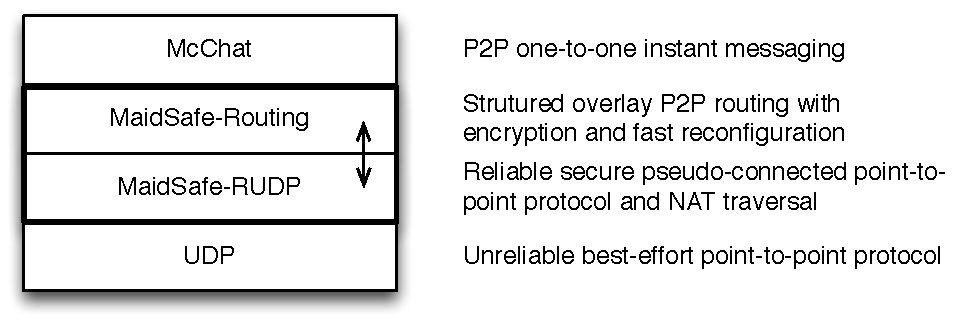
\includegraphics[width=0.8\textwidth]{figures/stack}
\caption[McChat network stack]{\label{fig:Stack} McChat network stack. The Routing and RUDP layers interact in both directions to provide their respective services: Routing uses RUDP for message sending and RUDP uses Routing for Network Address Translation (NAT) traversal when both nodes are behind symmetric NAT routers.}
\end{center}
\end{figure}

\subsection{Trust Model}

The security of an application is usually assessed against known forms of attacks. One key element of the analysis is which components of the system are trusted and for what operations. Since the aim of this report is not to assess the security of the Novinet libraries in a real-world situation, but still provide an interesting case study, the trust model that is going to be used assumes that all nodes on the network and the underlying machine on which they run can be trusted and will not be tampered. The storage medium that each user has for storing private data can also be trusted and can only be accessed by their owner. The communicating parties, Alice and Bob, can also trust one another. However, Eve is a malicious attacker and cannot be trusted, but she can only look at packets transmitted over the physical network, or interact with instant messaging network through the provided API. Since nodes are trusted, she will be assumed not to have tampered the node with which she can interact. The trust model is illustrated in Figure~\ref{fig:TrustModel}.. Needless to say, that scenario is not realistic but fully addressing the general case is beyond the scope of this report. 

\begin{figure}[htb]
\begin{center}
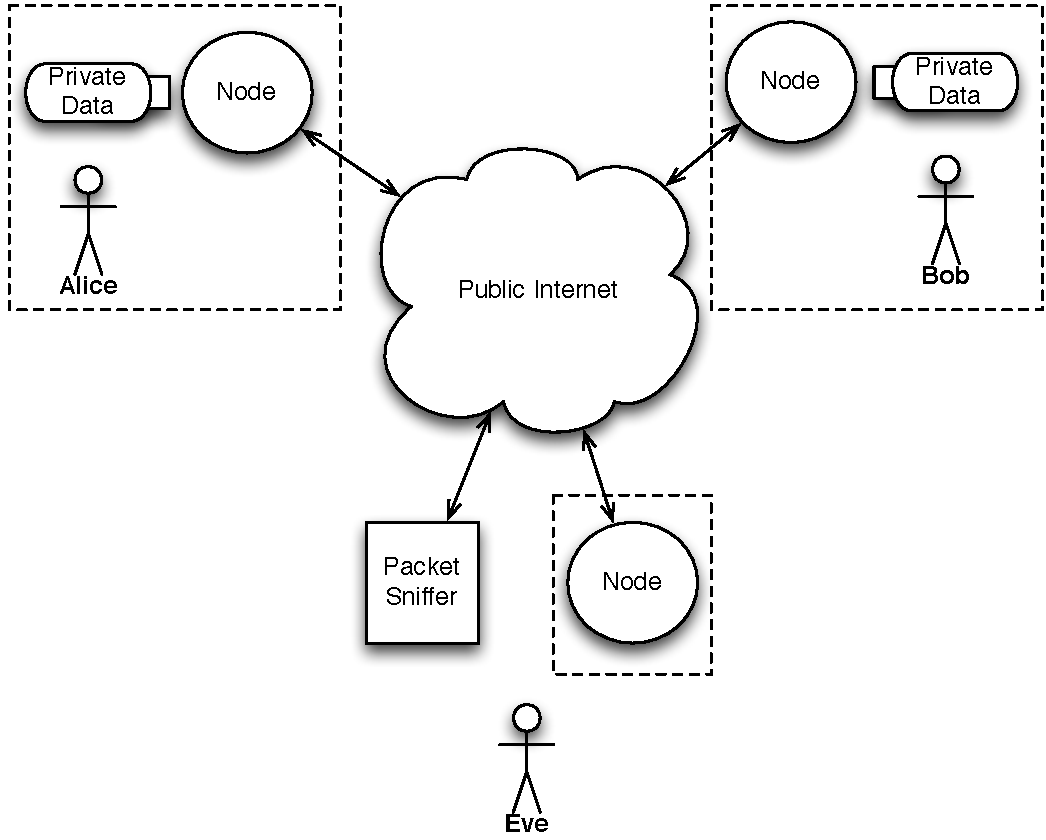
\includegraphics[width=0.8\textwidth]{figures/TrustModel}
\caption[Trust Model]{\label{fig:TrustModel} Trust Model. The elements in the dashed boxes are trusted: nodes behave strictly according to their intended behaviour and have not been tampered. Eve can only listen to arbitrary packets on the network and interact with the system according to the predefined operations.}
\end{center}
\end{figure}

\subsection{Operations}

This section defines the operations of the McChat layer. They are listed in Table~\ref{table:McChatAPI} by category, which are in turn ordered in the chronological order in which they happen, for a message to be sent.  

First, a node needs to join the network through a publicly available endpoint (IP address and port), that presumably became know through another channel of communication, such as email. This can be done before a user tries to connect to the network.

Second, the user sets the encrypted local storage file containing its private data by supplying the path at which the data is stored with setLocalStorage(Path). If no local storage file is owned, a new one can be created with newLocalStorage(Path).

Third, the user connects to the network by supplying a username and password, which unlocks its local storage file, giving to the node access to the private and public key representing the user identity. In the more secure version, the system creates a public and private key for each contact with which the use communicates. In the simpler version, a single private and public key are created, the latter being the same as the UserID. Once the node has access to the local storage, an arbitrary number of randomly chosen nodes provide a cryptographic challenge to test the user identity. If the test fails, the user is disconnected. Otherwise, a session object is returned which allows the user to manage its contact and send messages. The network implicitly stores the node location of the user and associate it with its UserID and the node connects with all the contact in the contact list and will generate status changed events when they connect or disconnect.

UserID can be created or deleted using the createID and deleteID methods. Multiple IDs can be stored in the same local storage.

Fourth, contact management and messaging can be interleaved. Contacts can be added or removed using their UserID (public key). Finally, messages can be sent using the UserID of the recipient. The SendCallback serves to notify that the message was successfully delivered or generates an error after a predefined amount of time. Messages can be received by supplying a callback.

Note that the operations abstract the node location on the network and only operate in terms of UserID. Also note that the Local Storage operations are only required because the Novinet Vault library was not available at the time of writing. Once it is, the private data will be stored on the network itself.

\begin{table}
\centering
\begin{tabular}{|l|c|l|p{8cm}|}
\hline
\textbf{Operation Category} & \textbf{Object Type} & \textbf{Method Signature}\\ 
\hline
Networking & Node & join(Endpoint)\\ 
\hline
Local Storage* & Node & setLocalStorage(Path)\\ 
 &  & newLocalStorage(Path)\\ 
\hline
Login & Node & connect(UserName, Password) [ returns Session ]\\ 
 & Session & disconnect()\\ 
 &  & createID(UserName, Password)\\ 
 &  & deleteID(UserName, Password)\\ 
\hline
Contact Management & Session & addContact(UserID)\\ 
 & & removeContact(UserID)\\ 
 & & \parbox{8cm}{onContactStatusChanged(\{ \\
 $~~~~$connected: StatusChangedCallback,\\
 $~~~~$disconnected: StatusChangedCallback \\
\})}\\ 
\hline
Messaging & Session & send(UserID, Message, SendCallback)\\ 
 &  & onMessageReceived(MessageReceivedCallback)\\ 
\hline\end{tabular}
\label{table:McChatAPI}
\caption[McChat API Summary]{McChat API summary: a Node object represents the current running node and is expected to be present as an object in the execution environment. A Session object is returned once a connection is successful. (*) Local Storage is only needed because MaidSafe Vaults were not available at the time of writing. Once available, they will be used to store user information on the network itself.}
\end{table}

The next chapter explains how these operations are implemented in terms of the Novinet library primitives and the procedure to bootstrap the network.
